\subsection{Problem definition}

This problem shows 1D heat transport by advection and diffusion in a $\unit[100]{m}$ long fracture. The fracture is fully saturated with groundwater, flowing with constant velocity. There is no rock matrix around the fracture which could store heat. Fig.~\ref{fig-addiff1} give a view about the situation.
\begin{figure}[h]
\centering
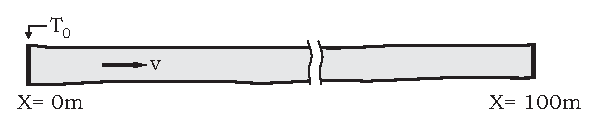
\includegraphics[width=0.5\textwidth]{T/figures/Ad-Diff-Problem-def.eps}
\caption{\label{fig-addiff1}A fully saturated fracture with flowing groundwater and a constant temperature at the left border.}
\end{figure}

%%%%%%%%%%%%%%%%%%%%%%%%%%%%%%%%%%%%%%%%%%%%%%%%%%%%%%%%%%%%%%%%%%%%%%%%%%%%%%%%%%%%%%%%%%%%%%%%%%%%%%%%%%%%%%%%%%%%
\subsection{Parameters}

The fracture is described as a porous medium with $\unit[100]{\%}$ porosity, so that no solid material influences the heat transport process. The properties of the fluid are in Tab.~\ref{tab-addiff}.
\begin{table}[h]
\caption{\label{tab-addiff}Material properties.}
\begin{center}
\begin{tabular}{ll}
\toprule
parameter 						& value \\
\midrule
density $\rho$ 					& $\unit[1000]{kg \cdot m^{-3}}$ \\			
thermal capacity $c$			& $\unit[4000]{J \cdot kg^{-1} \cdot K^{-1}}$ \\
thermal conductivity $\lambda$ 	& $\unit[0.6]{W \cdot m^{-1} \cdot K^{-1}}$ \\
\bottomrule
\end{tabular}
\end{center}
\end{table}
These values cause a diffusivity constant for water of $\alpha=\unit[1.5 \cdot 10^{-7}]{m^2/s}$. The groundwater velocity in the fracture is $v=\unit[3.0 \cdot 10^{-7}]{m^2/s}$.

%%%%%%%%%%%%%%%%%%%%%%%%%%%%%%%%%%%%%%%%%%%%%%%%%%%%%%%%%%%%%%%%%%%%%%%%%%%%%%%%%%%%%%%%%%%%%%%%%%%%%%%%%%%%%%%%%%%%%%
\subsection{Analytical solution}

For 1D-advective/diffusive transport, an analytical solution is given by \textsc{Ogata $\&$ Banks} as
\begin{equation}
T(x,t)=\frac{T_0}{2}\bigg( \operatorname{erfc} \frac{x-v_x\cdot t}{\sqrt{4\alpha t}} + e^{\frac{v_x\cdot x}{\alpha}} \operatorname{erfc}\frac{x+v_x\cdot t}{\sqrt{4\alpha t}}\bigg),
\label{eqn:addiff1}
\end{equation}
where $T_0$ is the constant temperature at $x=0$, $v$ is the groundwater velocity and $\alpha$ is the heat diffusivity coefficient of water (see \cite{HaeSamVoi:92},\cite{Kol:97}).

%%%%%%%%%%%%%%%%%%%%%%%%%%%%%%%%%%%%%%%%%%%%%%%%%%%%%%%%%%%%%%%%%%%%%%%%%%%%%%%%%%%%%%%%%%%%%%%%%%%%%%%%%%%%%%%%%%%%%%%
\subsection{Numerical solution}

The mesh for the numerical model consists of 501 nodes combining 500 line elements. The distance between the nodes is $\Delta x=\unit[0.2]{m}$.

\paragraph{Boundary conditions}
\begin{itemize}
	\item Left border:
	\begin{compactitem}
		\item constant source term (liquid flow) with $Q=\unit[3.0 \cdot 10^{-7}]{m^3/s}$
		\item constant temperature with $T=\unit[1]{^\circ C}$
	\end{compactitem}
	\item Right border:	
	\begin{compactitem}
		\item constant pressure with $P=\unit[100,000]{kPa}$
	\end{compactitem}
	\item Initial conditions:
	\begin{compactitem}
		\item pressure with $P=\unit[100,000.0]{kPa}$ for whole domain
		\item temperature $T=\unit[0]{^\circ C}$ for whole domain
	\end{compactitem}
	\item Time step:
	\begin{compactitem}
		\item $\Delta t=\unit[133,333.0]{s}$
	\end{compactitem}
\end{itemize}
With the given parameters, the \textsc{Neumann} criteria \eqref{eqn:ne-ldh} results on $\operatorname{Ne}=0.5$ which guarantees the numerical stability of the diffusion part of the transport process. The \textit{Courant} criteria, given by
\begin{equation}
	C=\frac{v_x\cdot\Delta t}{\Delta x}\leq1
	\label{eqn:addiff2}
\end{equation}\\
results to $C=0.2$.
%%%%%%%%%%%%%%%%%%%%%%%%%%%%%%%%%%%%%%%%%%%%%%%%%%%%%%%%%%%%%%%%%%%%%%%%%%%%%%%%%%%%%%%%%%%%%%%%%%%%%%%%%%%%%%%%%%%%%%%
\subsection{Results}

In Fig.~\ref{fig-addiff-re1} the comparison of analytical and numerical solution is plotted. The figure shows the temperature breakthrough curve at the end of the fracture at $x=\unit[100]{m}$. The numerical results show an acceptable agreement to the analytical solution. In a further step, the diffusion part of the heat transport process was avoided by minimizing the thermal conductivity of the fluid. Fig.~\ref{fig-addiff-re2} shows the breakthrough curve for only advective heat transport.
\begin{table}[h]
\caption{Benchmark deposit}
\begin{center}
\begin{tabular}{lll}
\toprule
Deposit & Version & Date \\
\midrule
T$\backslash$Ogata-Banks$\backslash$Ogata-Banks & 4.7.03 & Jul.~2008 \\
\bottomrule
\end{tabular}
\end{center}
\end{table}
\begin{figure}[H]
\centering
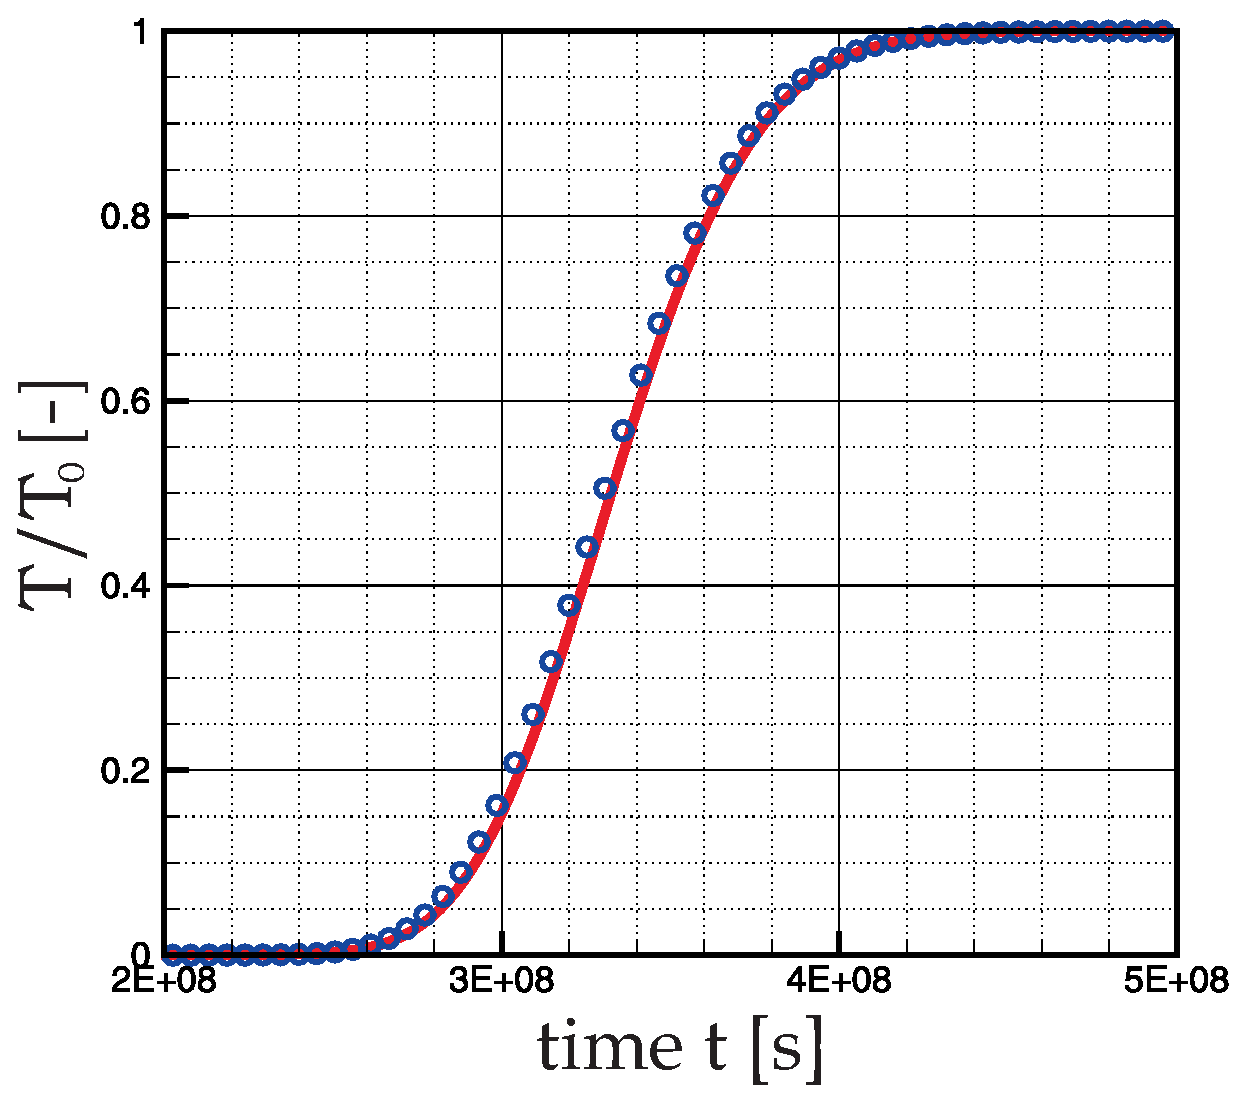
\includegraphics[width=0.5\textwidth]{T/figures/Ad-Diff.eps}
\caption{\label{fig-addiff-re1}Temperature breakthrough curve at the point $x=\unit[100]{m}$.}
\end{figure}
\begin{figure}[h]
\centering
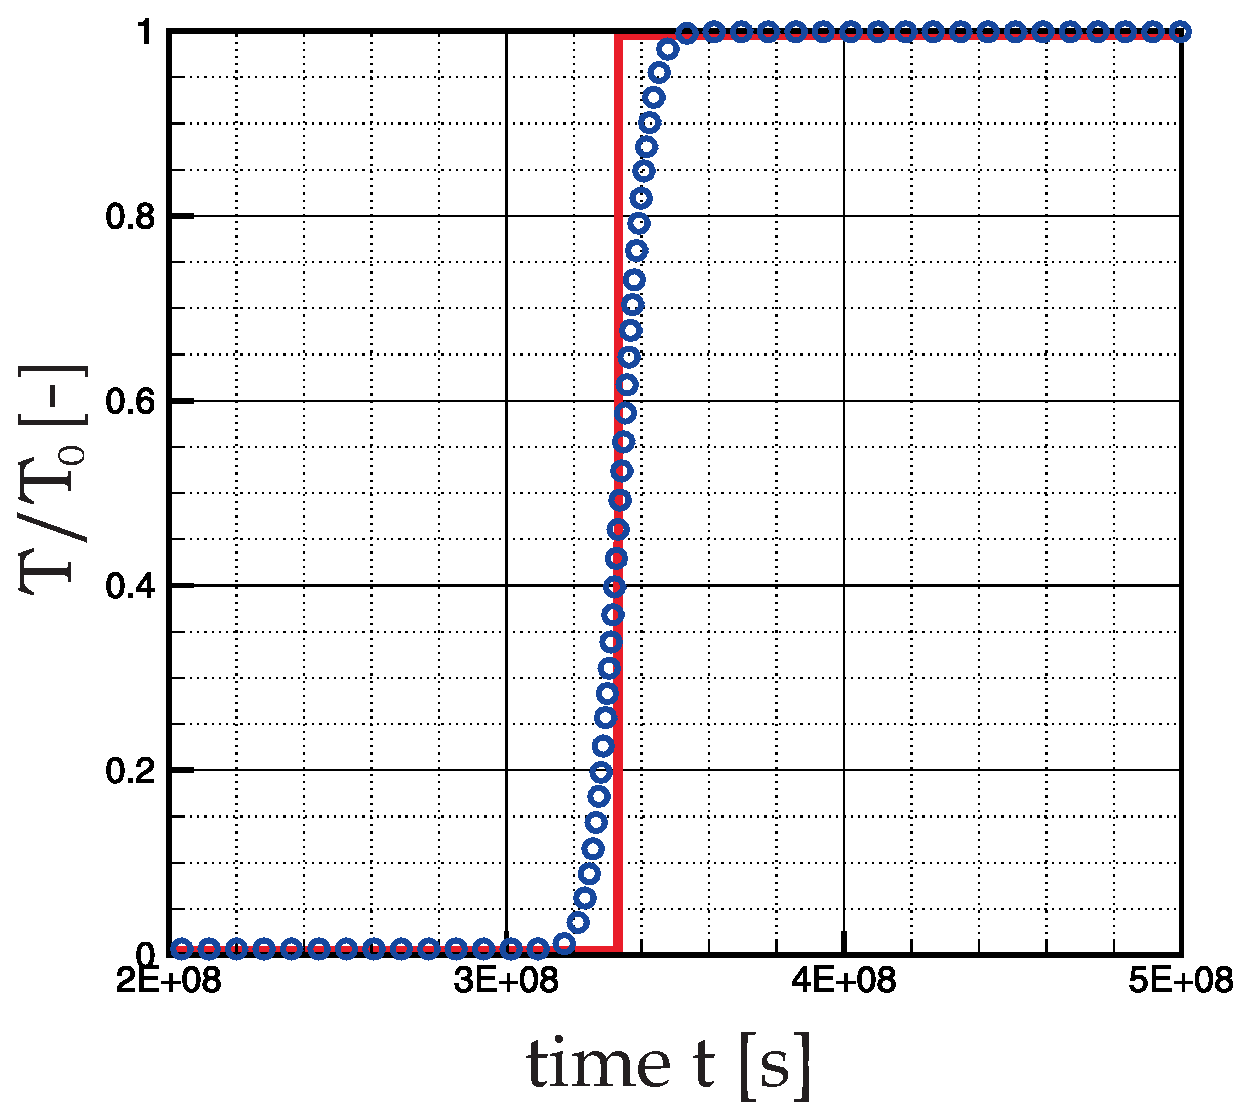
\includegraphics[width=0.5\textwidth]{T/figures/advection.eps}
\caption{\label{fig-addiff-re2}Temperature breakthrough curve when diffusion is avoided.}
\end{figure}
%\clearpage